\documentclass[tikz,border=5pt]{standalone}
\usepackage[utf8]{inputenc}
\usepackage[T1]{fontenc}
\usepackage{lmodern}
\usepackage{amsmath}
\usepackage{amssymb}
\usepackage{tikz}

\usepackage{xcolor}
\definecolor{black}{HTML}{000000}
\definecolor{white}{HTML}{FFFFFF}

\tikzset{
    scope_frame/.style={draw=black, fill=white, rounded corners=3pt, line width=0.85pt},
    scope_grid/.style={step=0.25cm, gray!25, very thin},
    scope_axis/.style={gray!70, thin},
    scope_wave/.style={draw=black, line width=1.15pt}
}

\begin{document}
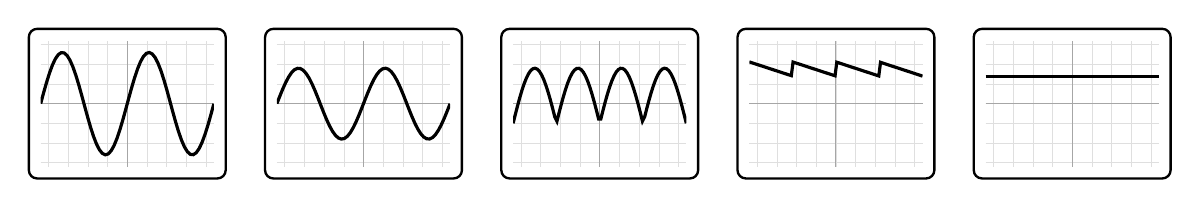
\begin{tikzpicture}
    % Macro Interna de Osciloscopio (Silencio Textual)
    \newcommand{\renderScope}[3]{
        \begin{scope}[shift={(#1,#2)}]
            \draw[scope_frame] (-1.25, -0.95) rectangle (1.25, 0.95);
            \draw[scope_grid] (-1.1, -0.8) grid (1.1, 0.8);
            \draw[scope_axis] (-1.1, 0) -- (1.1, 0);
            \draw[scope_axis] (0, -0.8) -- (0, 0.8);
            \begin{scope}
                \clip (-1.1, -0.8) rectangle (1.1, 0.8);
                #3
            \end{scope}
        \end{scope}
    }

    % Osciloscopio 1: Red AC
    \renderScope{0}{0}{
        \draw[scope_wave] plot[domain=-1.1:1.1, samples=60] (\x, {0.65*sin(360*\x/1.1)});
    }

    % Osciloscopio 2: Secundario Transformador
    \renderScope{3.0}{0}{
        \draw[scope_wave] plot[domain=-1.1:1.1, samples=60] (\x, {0.45*sin(360*\x/1.1)});
    }

    % Osciloscopio 3: Rectificación Onda Completa
    \renderScope{6.0}{0}{
        \draw[scope_wave] plot[domain=-1.1:1.1, samples=80] (\x, {0.70*abs(sin(360*\x/1.1)) - 0.25});
    }

    % Osciloscopio 4: Rizado y Filtrado Bulk
    \renderScope{9.0}{0}{
        \draw[scope_wave] plot[domain=-1.1:1.1, samples=100] (\x, {0.35 + 0.18*(1 - mod(\x+1.1, 0.55)/0.55)});
    }

    % Osciloscopio 5: Salida DC Regulada
    \renderScope{12.0}{0}{
        \draw[scope_wave] (-1.1, 0.35) -- (1.1, 0.35);
    }
\end{tikzpicture}
\end{document}
